% ============================================================
% CIC 2026 draft -- Springer LNCS (llncs) template
% Compile: latexmk -pdf main.tex
%
% All numbers in Sections 5-6 are REAL, taken from:
%   - training run  cnn_gru_spatial_softmax_robust_v9_20260714
%     (perturbation-aware augmentation: noise max 2.0 / drift max 2.0,
%      mutually exclusive per window; velocity loss weight 2.0)
%   - benchmark run robustness_benchmark_20260714_181137
%   - ablation variants: robustness_benchmark_20260709_154410 (no
%     perturbation-aware aug) and _154003 (GAP encoder, no geom aug)
% Everything still open is wrapped in \TBD{...} and is doable with
% the existing platform (mainly the planned user study in Sect. 7).
% ============================================================

\documentclass[runningheads]{llncs}

\usepackage[T1]{fontenc}
\usepackage{graphicx}
\usepackage{amsmath,amssymb}
\usepackage{booktabs}
\usepackage{url}
\usepackage{xcolor}
\usepackage{tikz}
\usetikzlibrary{arrows.meta,positioning,fit}

% Placeholder marker: red = still needs your input / future data.
\newcommand{\TBD}[1]{\textcolor{red}{\textbf{[#1]}}}

\begin{document}

\title{Reducing Cognitive Translation Cost in Embodied Tactile Robot
Control with a Learned Spatiotemporal Policy}
\titlerunning{Learned Embodied Tactile Control}

\author{First Author\inst{1}\orcidID{0000-0000-0000-0000} \and
Second Author\inst{1}\orcidID{0000-0000-0000-0000} \and
Third Author\inst{2}\orcidID{0000-0000-0000-0000}}
\authorrunning{F. Author et al.}

\institute{Department/Institute, Organization, City, Country\\
\email{corresponding.author@email.com} \and
Department/Institute, Organization, City, Country}

\maketitle

\begin{abstract}
When an operator guides a collaborative robot, the desired motion is
perceived directly at the robot body, yet conventional interfaces force
this spatial intention through a chain of symbolic translations---mode
selection, key lookup, coordinate-frame reasoning---before any motion
occurs. We frame this burden as \emph{cognitive translation cost} and
argue that an embodied tactile interface, where the operator slides a
finger over a capacitive skin on the robot itself, shortens the
intention-to-action pathway. That pathway, however, is only as strong as
its machine-decoding stage, which must remain trustworthy on a physical
sensor that drifts, ages, and breaks. The core contribution of this
paper is a learned decoder for this stage: from operator demonstration
sessions recorded directly on the platform, with no manual labeling, we
train a compact spatiotemporal policy that maps raw capacitance-map
sequences to velocity commands and interaction modes, using geometric
augmentation that exploits the sensor's physical symmetries and
perturbation-aware augmentation that corrupts the inputs while keeping
the command targets fixed. On a faithful-replay robustness benchmark
that streams identically perturbed episodes through unmodified deployed
implementations, the learned policy reproduces the demonstrated commands
on clean input and outperforms a conventional hand-crafted
centroid-tracking controller in every tested condition across four
perturbation families. A planned user study will quantify the remaining
human-side translation components against keyboard and teach-pendant
control.

\keywords{Human--robot interaction \and Embodied interaction \and Tactile
sensing \and Imitation learning \and Robustness evaluation \and Cognitive
translation cost}
\end{abstract}

% ==================================================================
\section{Introduction}
\label{sec:intro}

Collaborative robots are increasingly operated by people who stand next
to them. The operator sees, at the robot or the workpiece, exactly which
way the tool should move---yet most interfaces require that spatial
intention to be re-expressed symbolically: find the correct key or
pendant button, verify the coordinate frame, check the control mode,
then watch whether the response matches the intent. We use the term
\emph{cognitive translation cost} for the observable burden accumulated
along this intention-to-action pathway, measured through delays,
wrong-axis selections, mode transitions, corrective inputs, and response
latency (Sect.~\ref{sec:framework}).

An \emph{embodied} tactile interface attacks the translation problem at
its source: a capacitive skin wrapped around a robot link lets the
operator place a finger on the robot and slide it in the direction the
tool should move, so the command action is physically co-located with
the robot and spatially congruent with the intended motion
\cite{fitts1953}. But co-location only removes the \emph{human-side}
translation stages. The pathway still contains a machine-decoding stage
that converts raw taxel data into velocity commands, and conventional
implementations are hand-crafted pipelines of centroid tracking,
thresholds, and mode heuristics whose every parameter silently assumes a
clean, calibrated, undamaged sensor---while capacitive arrays drift,
taxels die, and gain varies across fabrication batches. An embodied
interface whose decoder misreads a degraded sensor does not reduce
translation cost; it merely relocates it into corrections and re-tries.

This paper therefore concentrates on the machine side of the pathway and
makes it \emph{learned, compact, and measurably robust}. Our
contributions are:

\begin{enumerate}
  \item \textbf{A conceptual framing} that decomposes the
  intention-to-action pathway into four observable translation components
  and locates the machine-decoding stage within it
  (Sect.~\ref{sec:framework}).
  \item \textbf{An automatic demonstration-recording pipeline}: labeled
  training episodes are logged as a by-product of normal use, with no
  manual labels (Sect.~\ref{sec:platform}).
  \item \textbf{A location-preserving learned policy}: a convolutional
  encoder with per-channel spatial softmax and a recurrent head, trained
  with geometry-aware and perturbation-aware augmentation that corrupts
  the inputs while keeping the command targets fixed
  (Sect.~\ref{sec:policy}).
  \item \textbf{A faithful-replay robustness benchmark} that scores
  unmodified deployed controller implementations under identical sensor
  corruptions, showing the learned policy outperforms a conventional
  hand-crafted centroid-tracking controller in every tested condition
  (Sects.~\ref{sec:benchmark}--\ref{sec:results}).
\end{enumerate}

A user study comparing the embodied interface against keyboard and
teach-pendant control is specified in Sect.~\ref{sec:userstudy}.

% ==================================================================
\section{Related Work}
\label{sec:related}

Human--robot interaction research has long examined how interfaces
bridge the gap between human intention and robot representation
\cite{goodrich2007,billard2019}: teach pendants provide structured
industrial control but require coordinate-frame interpretation, while
kinesthetic teaching reduces representational distance but depends on
backdrivability or force sensing. Spatial-compatibility research
supplies the underlying mechanism---responses are faster and less
error-prone when stimulus and response arrangements are spatially
congruent \cite{fitts1953}. Robot tactile sensing has meanwhile
progressed from discrete contact switches to conformal and textile
skins \cite{dahiya2010,si2023,luo2021}. Most systems treat touch as
information \emph{received} by the robot; a smaller body of work treats
it as an intentional command channel \cite{argall2010}, typically
realized with hand-crafted centroid-tracking controllers for continuous
velocity guidance. We are not aware of prior work that both learns this
mapping end-to-end from the raw taxel stream and quantifies its
robustness against the conventional controller design under identical
sensor corruptions.

Casting controller construction as supervised learning from recorded
demonstrations is a long-standing idea \cite{pomerleau1989,argall2009},
with well-understood strengths and caveats such as covariate shift
\cite{ross2011}. Here the demonstrations are recorded on the deployed
platform itself, so the training distribution matches deployment by
construction; the open question is generalization under \emph{input
corruption}, which is exactly what our benchmark measures.
Spatial-softmax feature points originate in end-to-end visuomotor
learning \cite{levine2016,finn2016}; we show they matter even on a
coarse taxel grid, where global pooling destroys the location
information that determines command direction.

Finally, aggregate outcomes such as completion time establish whether an
interface works, but compress several sources of inefficiency into one
number. Cognitive-infocommunications research argues for analyzing
human--machine systems through the structured interplay of their
cognitive capabilities rather than end-to-end scores alone
\cite{baranyi2012}, and corruption benchmarks report robustness per
perturbation family rather than as a single score \cite{hendrycks2019}.
We apply this principle to both the human side (observable translation
stages) and the machine side (robustness per perturbation family and
magnitude).

% ==================================================================
\section{Cognitive Translation-Cost Framework}
\label{sec:framework}

Let $I$ denote the user's intended robot motion, $D$ the
interface-compatible command decision, $U$ the physical input action, $C$
the machine-decoded command, $A$ the resulting robot action, and $F$ the
observable feedback:
\begin{equation}
I \rightarrow D \rightarrow U \rightarrow C \rightarrow A \rightarrow F.
\label{eq:pathway}
\end{equation}
Translation burden does not arise at a single point; different
interfaces load different stages (Fig.~\ref{fig:pathway}). Four
observable components summarize the pathway: \emph{mode-switching cost}
$M$ (interface-state transitions before a command can be issued),
\emph{command-production cost} $N$ (physical input events including
corrections), \emph{spatial-translation cost} $S$ (difficulty of mapping
a perceived task-space motion to the interface representation), and
\emph{feedback-closure cost} $L$ (delay from input to observable robot
response).

\begin{figure}[t]
\centering
\resizebox{\textwidth}{!}{%
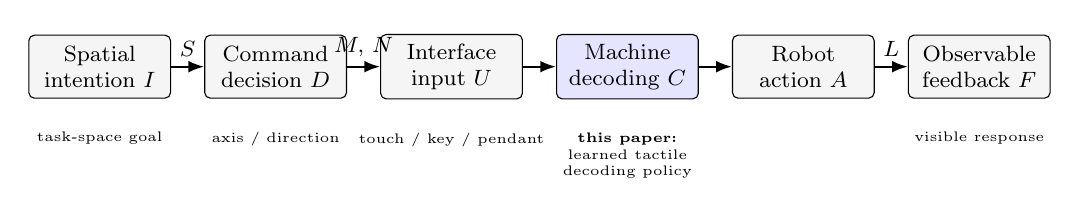
\begin{tikzpicture}[
    node distance=4.5mm and 4.2mm,
    stage/.style={draw, rounded corners=2pt, align=center, minimum height=8mm, minimum width=18mm, fill=gray!8, font=\footnotesize},
    hot/.style={draw, rounded corners=2pt, align=center, minimum height=8mm, minimum width=18mm, fill=blue!10, font=\footnotesize},
    cost/.style={align=center, font=\footnotesize\bfseries},
    arr/.style={-{Latex[length=2mm]}, thick}
]
\node[stage] (I) {Spatial\\intention $I$};
\node[stage, right=of I] (D) {Command\\decision $D$};
\node[stage, right=of D] (U) {Interface\\input $U$};
\node[hot, right=of U] (C) {Machine\\decoding $C$};
\node[stage, right=of C] (A) {Robot\\action $A$};
\node[stage, right=of A] (F) {Observable\\feedback $F$};

\draw[arr] (I) -- node[cost, above] {$S$} (D);
\draw[arr] (D) -- node[cost, above] {$M,\,N$} (U);
\draw[arr] (U) -- (C);
\draw[arr] (C) -- (A);
\draw[arr] (A) -- node[cost, above] {$L$} (F);

\node[font=\tiny, align=center, below=3mm of I] {task-space goal};
\node[font=\tiny, align=center, below=3mm of D] {axis / direction};
\node[font=\tiny, align=center, below=3mm of U] {touch / key / pendant};
\node[font=\tiny, align=center, below=3mm of C] {\textbf{this paper:}\\learned tactile\\decoding policy};
\node[font=\tiny, align=center, below=3mm of F] {visible response};
\end{tikzpicture}%
}
\caption{Intention-to-action pathway. Embodied tactile input targets the
human-side costs $S$, $M$, and $N$; this paper concentrates on the
highlighted machine-decoding stage $U \rightarrow C$, whose brittleness
under sensor degradation would re-enter the pathway as corrective
inputs.}
\label{fig:pathway}
\end{figure}

For keyboard and pendant interfaces the decoding stage is trivial---a key
press is unambiguous---and translation cost concentrates in $S$, $M$, and
$N$. An embodied tactile interface inverts this distribution: touching
the robot where motion should occur makes $S$ nearly free and collapses
mode navigation, but decoding becomes a perception problem on a physical
sensor that drifts, ages, and breaks. Reliability of stage $C$ is thus
the condition under which the embodied interface's human-side advantage
survives contact with reality; it motivates the learned decoder and the
explicit robustness benchmark that follow.

% ==================================================================
\section{Embodied Tactile Platform and Demonstration Data}
\label{sec:platform}

The testbed is a woven capacitive tactile skin providing an $n \times m$
grid of taxels, mounted on the end link of a 6-DOF collaborative arm
(TM5-900); interlaced conductive threads conform to the curved robot
geometry. Per frame the skin outputs a matrix of relative capacitance
changes against a per-session calibration baseline; touch produces
negative deviations roughly proportional to contact pressure. A short
moving average is computed alongside the instantaneous signal, and
frames are consumed at approximately 60\,Hz. The command vocabulary
covers task-space translation driven by finger motion, plus two
pressure-gated modes: a hard press commands a \emph{push} along $+v_y$
and a two-finger pinch commands a \emph{pull} along $-v_y$.
\TBD{One to two sentences on skin construction and readout electronics,
with a citation to the hardware publication if available.}

\label{sec:data}
During demonstration sessions an operator guides the end-effector by
interacting freely with the skin, and at each control tick the platform
automatically records the instantaneous and averaged capacitance
matrices, the commanded 6-DOF end-effector velocity, the interaction
mode $m_t^\ast \in \{\textit{stop}, \textit{move}, \textit{push},
\textit{pull}\}$, and lightweight contact descriptors computed from the
touch map (centroid, displacement, speed, peak and mean pressure, touch
presence). Labeled training episodes are thus a by-product of normal
operation; no frame was manually annotated. The corpus comprises eight
episodes---roughly five minutes of continuous interaction---across a
free-swiping session and a push/pull-focused session. Rotational axes
were not exercised and are locked to zero throughout.

% ==================================================================
\section{Learned Decoding Policy}
\label{sec:policy}

\subsection{Input Representation and Architecture}

The policy consumes a sliding window of recent frames, each a 4-channel
$n \times m$ image: the instantaneous capacitance deviation, its moving
average, the temporal difference between consecutive frames, and a
binary touch mask obtained by thresholding the averaged channel. A
compact auxiliary vector carries the contact descriptors of
Sect.~\ref{sec:data}, which summarize contact geometry while the raw
frames preserve everything they discard.

A stack of $3\times3$ convolutions processes each frame at full taxel
resolution---no spatial pooling at any depth. A per-channel
\emph{spatial softmax} then reduces each feature map
$F_k \in \mathbb{R}^{n\times m}$ to its expected image coordinate,
\begin{equation}
\mathbf{p}_k = \sum_{(i,j)}
\operatorname{softmax}\!\big(F_k/\theta\big)_{ij}\,(u_i, u_j),
\qquad u \in [-1, 1],
\label{eq:ssoftmax}
\end{equation}
with a learned temperature $\theta$. Concatenating the keypoints with
the per-channel mean intensities yields a frame descriptor that
preserves \emph{where} the contact is and \emph{how hard} it presses;
the common alternative, global average pooling, collapses location
entirely, and Sect.~\ref{sec:results-ablation} quantifies its cost.
Frame descriptors are fused with an encoding of the auxiliary vector and
passed through a single-layer GRU, whose final hidden state feeds a
velocity-regression head and a mode classifier. The model is compact and
its per-window CPU inference time sits an order of magnitude inside the
60\,Hz control budget, contributing negligibly to the feedback-closure
cost $L$.

\subsection{Geometry- and Perturbation-Aware Augmentation}
\label{sec:augment}

Five minutes of demonstration cannot cover the product space of contact
locations, directions, and pressures---but the sensor's geometry provides
exact symmetries. During training each sampled window is randomly
\emph{flipped} on the taxel grid, with the transformation propagated
consistently through every affected quantity (a column flip negates
$v_x$ and mirrors the column-related contact descriptors; a row flip
acts analogously on $v_z$), and \emph{translated} by a small random
offset bounded so that no active cell leaves the grid. Flips multiply
directional coverage by four; translation decouples the mapping from
absolute contact position; mode labels are invariant throughout.

A second, \emph{perturbation-aware} scheme targets sensor degradation
directly. For a random subset of training windows, one of two corruption
modes is sampled, mirroring the one-failure-at-a-time structure of the
benchmark: either i.i.d.\ Gaussian noise of a randomly drawn magnitude,
injected exactly as physical noise would propagate through the sensing
pipeline (raw noise into the instantaneous channel, its moving average
into the averaged channel, its delta into the temporal-difference
channel, and the touch mask recomputed from the corrupted average), or a
randomly drawn baseline offset that emulates calibration drift.
Applying at most one corruption family per window
proved important: stacking noise and drift compounds the ambiguity and
makes the policy hedge its velocity magnitudes even on clean input.
Crucially, the velocity and mode \emph{targets are left unchanged}---the
operator's finger is doing the same thing regardless of sensor
health---so the policy learns to decode the same intent from a degraded
stream; Sect.~\ref{sec:results-ablation} shows this is what closes the
noise-robustness gap. Augmentation is never applied to validation data.

\subsection{Training Protocol}

Windows are split by \emph{episode}: six episodes train, two held-out
episodes (one per session) validate, and normalization statistics use
training data only. The loss combines a Smooth-$L_1$ velocity term with
a class-balanced cross-entropy mode term, weighted per sample to
de-emphasize \emph{stop} frames and emphasize the rare \emph{pull}
class; training uses AdamW with plateau-based decay and early stopping.

% ==================================================================
\section{Faithful-Replay Robustness Benchmark}
\label{sec:benchmark}

The benchmark answers one question: \emph{when the sensor misbehaves,
which decoder keeps translating operator intent correctly?} The learned
policy is compared against a conventional \textbf{hand-crafted
centroid-tracking controller}, representative of how continuous tactile
guidance is normally implemented: contacted taxels are clustered, a
pressure-weighted centroid is tracked with hysteresis and deadbanding
into velocity, and pressure-gated heuristics arbitrate the push/pull
modes---dozens of tuned parameters, each silently assuming a healthy
sensor. Three design decisions distinguish the benchmark.

\emph{(1) Deployed implementations, not re-implementations.} Recorded
episodes are streamed frame-by-frame into a sensor-emulation layer, and
both controllers run through their unmodified runtime classes, with all
stateful machinery, buffering, normalization, and confidence gating.

\emph{(2) Ground truth from clean input.} The reference at frame $t$ is
the command recorded on the \emph{clean} sensor stream, while both
controllers receive an identically \emph{perturbed} stream; a controller
scores well if corruption does not change what it believes the operator
wants.

\emph{(3) Self-validation.} At zero perturbation the replay harness
reproduces the commands recorded live on the held-out episodes, closing
the loop on harness fidelity before any perturbation is trusted.

Four perturbation families model the dominant failure modes of
capacitive arrays, injected consistently into both the instantaneous and
moving-average channels at mild and severe operating levels:
\textbf{baseline drift}, a uniform offset that emulates
thermal/humidity drift between calibrations (beyond the severe level,
idle cells begin to register as touched and sensing fails for any
decoder); \textbf{dead taxels}, a random fraction of cells clamped to
zero (up to 20\%); \textbf{gain error}, multiplicative scaling
(0.5--1.3$\times$); and \textbf{Gaussian noise}, i.i.d.\ per-cell
interference. Velocity error is reported as linear-axis RMSE against
the clean-input reference command; mode agreement as the fraction of
frames whose canonical mode matches.

% ==================================================================
\section{Results}
\label{sec:results}

\subsection{Fidelity to the Demonstrated Commands}

\begin{figure}[t]
\centering

\includegraphics[width=0.67\textwidth]{figure/validation_velocity_timeseries.png}
\caption{Predicted vs.\ demonstrated velocity on a held-out validation
segment ($v_x$, $v_y$, $v_z$ from top to bottom). The policy reproduces
direction changes on all three axes, push/pull events ($v_y$), and stop
phases.}
\label{fig:timeseries}
\end{figure}

On the two held-out episodes the policy attains a linear-velocity RMSE
of \textbf{1.55\,cm/s} against demonstrated commands whose magnitudes
reach 10\,cm/s, and \textbf{92.6\%} mode accuracy; mode confusions
concentrate where the demonstrations themselves are
ambiguous---\textit{stop} frames bordering \textit{push} onsets
(Fig.~\ref{fig:timeseries}). The policy thus faithfully reproduces the
demonstrated behavior on clean input; whether it holds on a degraded
sensor is answered next.

\subsection{Robustness under Sensor Perturbation}
\label{sec:results-robust}

\begin{table}[t]
\centering
\caption{Faithful-replay benchmark on held-out episodes: velocity RMSE
(m/s, lower is better) and mode agreement (higher is better) against the
clean-input reference. Bold marks the better controller per condition.}
\label{tab:robust}
\begin{tabular}{llcccc}
\toprule
& & \multicolumn{2}{c}{RMSE (m/s)} & \multicolumn{2}{c}{Mode agree.} \\
\cmidrule(lr){3-4}\cmidrule(lr){5-6}
Perturbation & Level & Centroid & Learned & Centroid & Learned \\
\midrule
None (clean)     & --      & 0.032 & \textbf{0.015} & 0.68 & \textbf{0.93} \\
\midrule
Baseline drift   & mild    & 0.032 & \textbf{0.017} & 0.69 & \textbf{0.91} \\
                 & severe  & 0.033 & \textbf{0.018} & 0.71 & \textbf{0.91} \\
\midrule
Dead taxels      & 10\%    & 0.032 & \textbf{0.015} & 0.68 & \textbf{0.93} \\
                 & 20\%    & 0.034 & \textbf{0.018} & 0.66 & \textbf{0.91} \\
\midrule
Gain error       & 0.7$\times$ & 0.036 & \textbf{0.019} & 0.61 & \textbf{0.90} \\
                 & 1.3$\times$ & 0.029 & \textbf{0.016} & 0.75 & \textbf{0.92} \\
\midrule
Gaussian noise   & mild    & 0.034 & \textbf{0.018} & 0.66 & \textbf{0.90} \\
                 & severe  & 0.040 & \textbf{0.031} & 0.66 & \textbf{0.75} \\
\bottomrule
\end{tabular}
\end{table}

\begin{figure}[t]
\centering

\includegraphics[width=0.7\textwidth]{figure/rmse_vs_perturbation.png}
\caption{Velocity RMSE vs.\ perturbation magnitude for both controllers.
Green shading marks conditions where the learned policy has the lower
error: every tested condition of all four families.}
\label{fig:robust}
\end{figure}

Table~\ref{tab:robust} and Fig.~\ref{fig:robust} report the benchmark.

\emph{The learned policy wins every tested condition.} Across all four
perturbation families and all magnitudes, the policy's velocity error
stays well below the centroid controller's, and its mode agreement stays
above it throughout. Under baseline drift the policy's error barely
rises; with one in five taxels dead it is nearly unchanged---the
convolutional encoder interpolates around missing cells, whereas a
pressure-weighted centroid has no such mechanism. The centroid
controller's modest mode agreement even on clean input is not a replay
error: the recorded reference captures the operator's \emph{intended}
interaction, which the heuristics do not always match.

\emph{Noise robustness had to be trained, not assumed.} Uncorrelated
per-frame noise is structurally hostile to this input representation:
the temporal-difference channel doubles the variance of i.i.d.\ noise
and the binary touch mask flickers under borderline contact readings,
while the centroid controller is partially shielded by reading only the
moving average. A variant trained \emph{without} perturbation-aware
augmentation indeed falls behind the centroid controller under noise
(Sect.~\ref{sec:results-ablation}); injecting sensor-consistent noise
and drift during training closes this gap completely, at almost no cost
on clean input.

\subsection{Ablation: Location-Preserving Encoding and Augmentation}
\label{sec:results-ablation}

\begin{table}[t]
\centering
\caption{Ablation on robustness (velocity RMSE, m/s; lower is better);
each row adds one ingredient. The hand-crafted centroid controller
scores 0.033--0.034 under these noise conditions. \TBD{Re-run the first
row as a controlled single-variable ablation before submission.}}
\label{tab:ablation}
\begin{tabular}{lcccc}
\toprule
Variant & Clean & Mild noise & Stronger noise & Dead 20\% \\
\midrule
GAP encoder, no geom.\ aug. & \textbf{0.014} & 0.055 & 0.059 & 0.022 \\
+ spatial softmax, geom.\ aug. & \textbf{0.014} & 0.033 & 0.043 & 0.019 \\
+ perturbation-aware aug.\ (ours) & 0.015 & \textbf{0.016} & \textbf{0.018} & \textbf{0.018} \\
\bottomrule
\end{tabular}
\end{table}

Table~\ref{tab:ablation} isolates each design choice. Clean-input
fidelity is essentially identical across all three variants---an
evaluation reporting only clean held-out metrics would find nothing to
choose between them. Under perturbation the differences are large: the
location-preserving encoder and geometric augmentation cut the
noise-induced error by roughly 40\% relative to global average pooling
but still trail the hand-crafted controller under noise, and
perturbation-aware augmentation closes the remaining gap and reverses
it at a negligible cost in clean RMSE. Robustness, not clean accuracy,
is where these design choices pay off.

% ==================================================================
\section{Planned User Evaluation}
\label{sec:userstudy}

The results above establish that the machine-decoding stage is robust
enough to carry a user-facing comparison. A ready-to-run protocol will
quantify the human-side components: three matched interfaces---embodied
tactile control using the learned policy, a keyboard, and the teach
pendant---issue the same bounded velocity primitives, with randomized
spatial command translation as the primary task and short multi-command
sequences as a secondary task. The principal measure is
intention-to-command initiation latency, complemented by first-input
correctness and wrong-axis selections ($S$), interface-state transitions
($M$), corrective inputs ($N$), and input-to-motion delay ($L$),
reported as a profile that preserves \emph{where} each interface loads
the pathway. A sub-condition with a masked-off taxel region will test
whether decoder degradation manifests as increased correction burden.
\TBD{Effect sizes, participant count, and statistics after data
collection.}

% ==================================================================
\section{Limitations and Conclusion}
\label{sec:conclusion}

Learning from demonstration reproduces the demonstrated strategy rather
than discovering better ones; our claim is robustness under corruption,
not superiority of the strategy itself. The augmentation uses i.i.d.\
noise and uniform drift; correlated noise models fitted to the physical
sensor are a natural refinement. All robustness results are open-loop
replay, a gap the user study closes. Rotational axes were locked to
zero, and results come from a single sensor unit and few operators.

In sum, an embodied tactile interface shortens the human side of the
intention-to-action pathway, but its promise rests on the
machine-decoding stage remaining trustworthy when the sensor does not.
We showed that this stage can be learned directly from operator
demonstrations recorded on the platform, and that the resulting policy
outperforms a conventional hand-crafted centroid-tracking controller in
every tested condition across all four perturbation families. The
methodological lesson from the ablation: this robustness was invisible
to clean held-out evaluation and had to be created deliberately, by
corrupting training inputs while holding the command targets fixed. A
decoder that holds its ground under sensor degradation is what keeps
the embodied interface's cognitive advantage intact.

% ==================================================================
\subsubsection{Acknowledgements.}
\TBD{Funding sources.}

\subsubsection{Disclosure of Interests.}
\TBD{No competing interests. (Adjust as required.)}

% ------------------------------------------------------------------
\begin{thebibliography}{14}

\bibitem{goodrich2007}
Goodrich, M.A., Schultz, A.C.: Human--robot interaction: a survey.
Foundations and Trends in Human--Computer Interaction 1(3), 203--275
(2007)

\bibitem{billard2019}
Billard, A., Kragic, D.: Trends and challenges in robot manipulation.
Science 364(6446), eaat8414 (2019)

\bibitem{fitts1953}
Fitts, P.M., Seeger, C.M.: S--R compatibility: spatial characteristics of
stimulus and response codes. Journal of Experimental Psychology 46(3),
199--210 (1953)

\bibitem{dahiya2010}
Dahiya, R.S., Metta, G., Valle, M., Sandini, G.: Tactile sensing: from
humans to humanoids. IEEE Transactions on Robotics 26(1), 1--20 (2010)

\bibitem{si2023}
Si, Z., Yu, T.C., Morozov, K., McCann, J., Yuan, W.: RobotSweater:
scalable, generalizable, and customizable machine-knitted tactile skins
for robots. In: IEEE International Conference on Robotics and Automation
(ICRA) (2023)

\bibitem{luo2021}
Luo, Y., Li, Y., Sharma, P., Shou, W., Wu, K., Foshey, M., Li, B.,
Palacios, T., Torralba, A., Matusik, W.: Learning human--environment
interactions using conformal tactile textiles. Nature Electronics 4(3),
193--201 (2021)

\bibitem{argall2010}
Argall, B.D., Billard, A.G.: A survey of tactile human--robot
interactions. Robotics and Autonomous Systems 58(10), 1159--1176 (2010)

\bibitem{pomerleau1989}
Pomerleau, D.A.: ALVINN: an autonomous land vehicle in a neural network.
In: Advances in Neural Information Processing Systems, pp. 305--313
(1989)

\bibitem{argall2009}
Argall, B.D., Chernova, S., Veloso, M., Browning, B.: A survey of robot
learning from demonstration. Robotics and Autonomous Systems 57(5),
469--483 (2009)

\bibitem{ross2011}
Ross, S., Gordon, G., Bagnell, D.: A reduction of imitation learning and
structured prediction to no-regret online learning. In: International
Conference on Artificial Intelligence and Statistics, pp. 627--635 (2011)

\bibitem{levine2016}
Levine, S., Finn, C., Darrell, T., Abbeel, P.: End-to-end training of
deep visuomotor policies. Journal of Machine Learning Research 17(39),
1--40 (2016)

\bibitem{finn2016}
Finn, C., Tan, X.Y., Duan, Y., Darrell, T., Levine, S., Abbeel, P.: Deep
spatial autoencoders for visuomotor learning. In: IEEE International
Conference on Robotics and Automation (ICRA), pp. 512--519 (2016)

\bibitem{hendrycks2019}
Hendrycks, D., Dietterich, T.: Benchmarking neural network robustness to
common corruptions and perturbations. In: International Conference on
Learning Representations (2019)

\bibitem{baranyi2012}
Baranyi, P., Csap\'o, \'A.: Definition and synergies of cognitive
infocommunications. Acta Polytechnica Hungarica 9(1), 67--83 (2012)

\end{thebibliography}

\end{document}
